\documentclass[12pt]{book}
\usepackage[utf8]{inputenc}
\usepackage{hyperref}
\usepackage{graphicx}
\usepackage{hyperref}
\usepackage{subcaption}

\title{Petit guide d'utilisation de Linux Mint}
\author{Association Eisenia}
\date{2021}

\begin{document}
\maketitle

\newpage
\renewcommand{\contentsname}{Table des matières}
\tableofcontents

\renewcommand{\chaptername}{Chapitre}
\chapter{Introduction}
%\section{Introduction générale}
Linux Mint est système d'exploitation.
Cela signifie qu'il fait le rôle d'interface entre l'utilisateur et la machine.
Il va permettre aux utilisateurs de lancer des programmes.
Le rôle du système d'exploitation est multiple.
Il existe beaucoup de systèmes d'exploitation différents, ici nous traiterons uniquement du système Linux Mint.
%\section{Introduction au logiciel libre}
Linux Mint est système d'exploitation libre.
C'est-à-dire, que son code est entièrement ouvert à qui veut le consulter.
Cela signifie également que tout utilisateur peut soumettre un changement dans le code du système d'exploitation.\par
Le "libre" s'oppose au "propriétaire".
Le propriétaire siginifie que le code appartient à une entreprise privée.
Le code n'est donc pas consultable et le propriétaire est le seul décisionnaire de ce qu'il peut y mettre.\par
Même si vous ne comprenez pas ou que vous ne voulez pas vous embêter à fouiller dans, parfois, des milliers de lignes de code, le libre vous garantie une protection de vos données, une transparence sur ce qui est fait.
Le libre étant développée par la communauté, il n'y a pas d'intérêt financier à concerver et vendre vos informations.\par
Dans ce livret, nous allons explorer Linux Mint.
Nous verrons les bases de ce système d'exploitation.
Nous aborderons aussi d'autres thématiques comme l'utilisation d'Internet et les bons gestes à aborder pour garder son ordinateur en bon état le plus longtemps possible.


\chapter{Environnement Linux Mint}
\begin{minipage}[c]{.25\textwidth}
	\centering
	
\includegraphics[width=.85\textwidth]{include/lm_logo.png}
%	\caption{Caption1}
%	\label{fig:wrapfig}
\end{minipage}
\begin{minipage}[c]{.75\textwidth}
	Linux Mint est un système d'exploitation visant à être utilisé facilement par les particuliers et les professionnels.
	C'est un systèmes d'exploitation libre et gratuit assez récent s'appuyer sur d'autres systèmes d'exploitation de Linux (Ubuntu/Debian).
\end{minipage}\par
Le but principal de Linux Mint est de Linux Mint est de faciliter au maximum l'utilisation d'un ordinateur pour le grand public.\par
Dans ce chapitre, nous intéresser aux bzses du système d'exploitation Linux Mint et plus particulièrement à son environnement de bureau appelé Cinnamon.
\section{Se familiariser avec l'environnement de bureau Cinnamon de Linux Mint}
	Pour bien commencer avec un nouvel envrironnement, il faut en connaître les bases.
	Savoir bien appréhender les bases de l'environnement, c'est mieux le comprendre et ainsi l'utiliser plus simplement, plus rapidement et se sentir plus à l'aise avec son matériel.\par
	Dans cette section nous allons voir les éléments basics pour bien commencer avec ce nouvel environnement de travail.
	\subsection{Le bureau}\label{sec:bureau}
		Le bureau est le premier élément qui s'affiche sur votre écran une fois votre session ouverte.
		C'est en quelque sorte votre écran d'accueil.
		Il contient des raccourcis vers des fichiers, des dossiers ou encore des applications que vous utilisés fréquement.
		\begin{figure}[h]
			\centering
			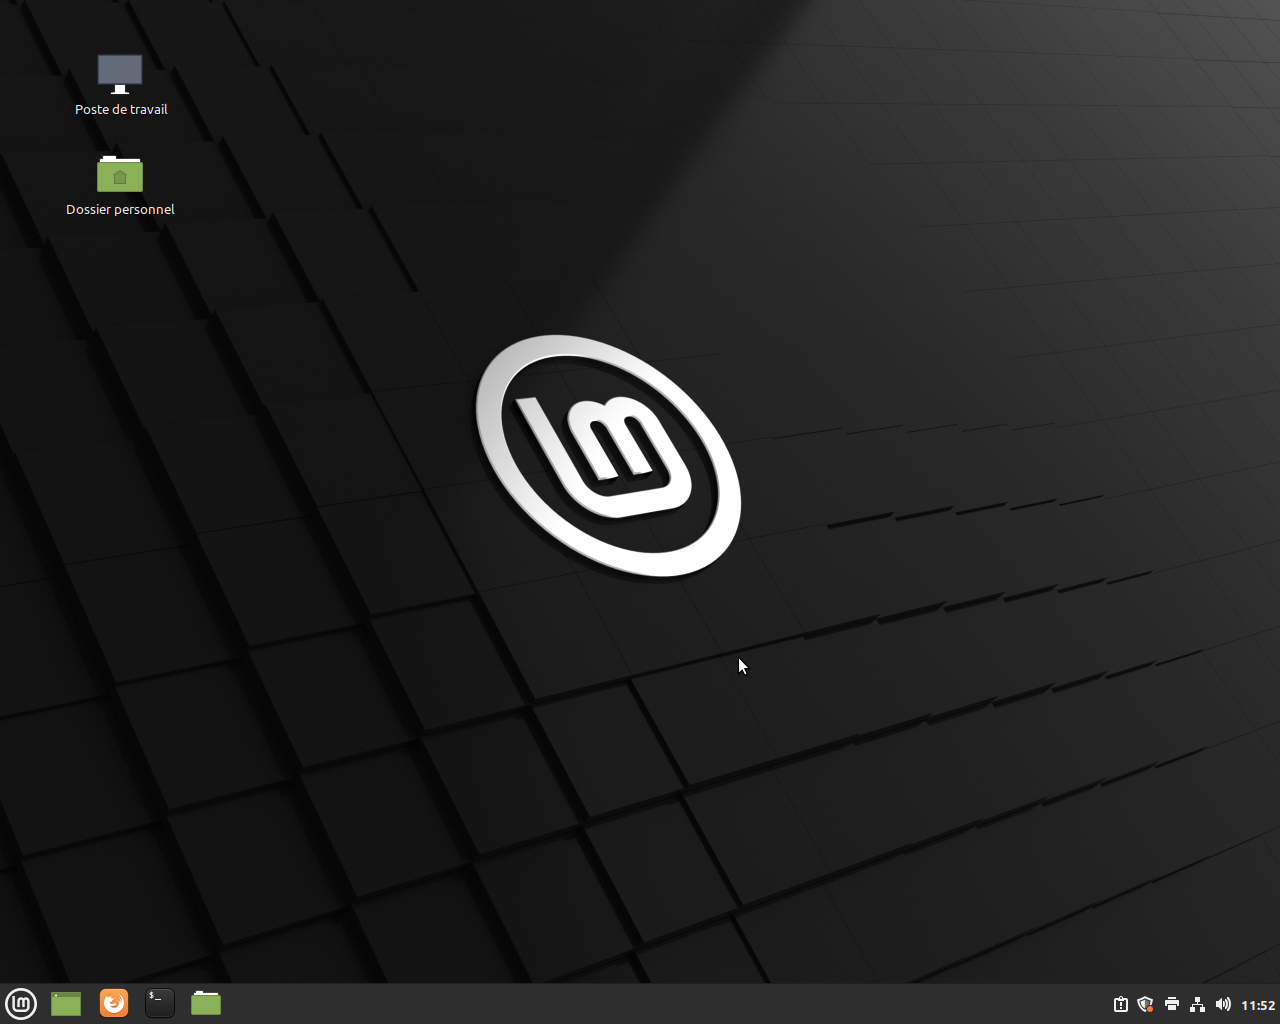
\includegraphics[width=\textwidth]{include/bureau.png}
			\caption{Bureau Linux Mint 20}
			\label{fig:bureau}
		\end{figure}\par
		Le but du bureau est de vous faciliter les choses.
		Vous pouvez donc le personnaliser à votre convenance.
		Nous allons voir comment nous pouvons changer le fond d'écran du bureau et comment ajouter et supprimer des éléments sur le bureau.
		\subsubsection{Changement du fond d'écran du bureau}
			Le fond d'écran du bureau est la première chose que l'on voit lorsque l'oon allume l'ordinateur.
			Il est donc préférable que ce fond d'écran nous plaise.\par
			Que vous ayez une image en tête ou bien que vous souhaitiez tout simplement consulter la banque d'image de fonds d'écran proposé sur votre ordinateur, vous pouvez faire ceci :
			\begin{enumerate}
				\item Sur le bureau, faire clic droit;
				\item Sélectionner "\texttt{Modifier l'arrière-plan du bureau}";
				\item Une sélection de fonds d'écran vous est proposé. Cliquez sur le fond d'écran qui vous intéresse et il sera immédiatement défini comme fond d'écran du bureau.
				\begin{figure}[h]
					\centering
					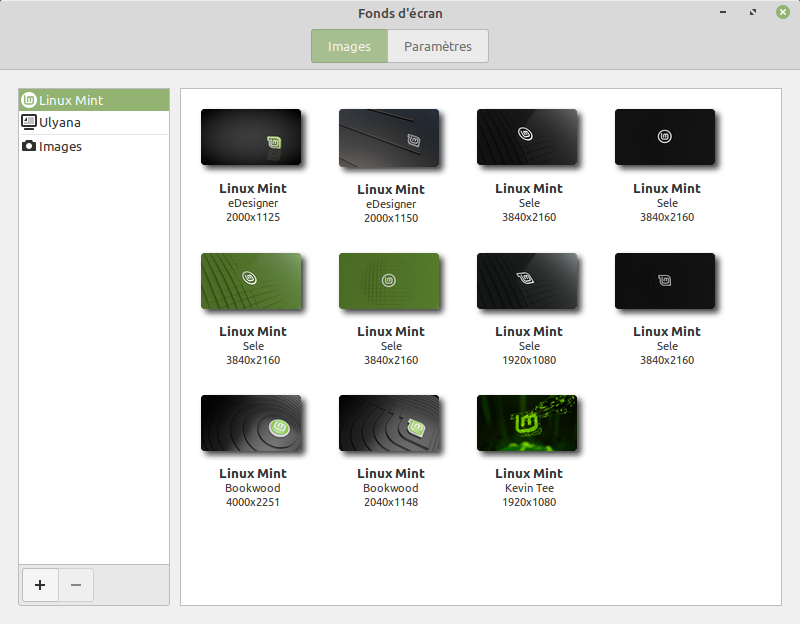
\includegraphics[width=\textwidth]{include/fondsdecran.png}
					\caption{Fenêtre pour sélectionner un nouveau fond d'écran}
					\label{fig:fondsdecran}
				\end{figure}\newline
				Sur le volet gauche de cette fenêtre, vous pouvez cliquez sur l'onglet "images" pour accéder aux images que vous avez enregistrées dans le dossier "Images" de votre ordinateur.
			\end{enumerate}
		\subsubsection{Ajout / suppression d'éléments sur le bureau}\label{sec:elementsbureau}
			Si vous utilisez très fréquement un fichier ou un logiciel et que vous ne voulez pas avoir à le chercher à chaque démarrage de votre machine, vous pouvez le mettre sur le bureau. Une petite icône sera alors ajouter au bureau en tant que "raccourcis" vers cet élément. 
			Ainsi, vous n'aurez qu'à cliquer sur cette icône pour ouvrir vos fichiers, vos dossiers ou vos applications favoris.\newline
			Pour mettre un nouvel élément sur votre bureau :
			\begin{enumerate}
				\item Faire clic droit sur l'élément;
				\item Sélectionner "\texttt{Ajouter au bureau}";
				\item Un raccourci a été ajouté sur votre bureau.
			\end{enumerate}\par
			Si vous ne souhaitez plus voir un élément sur votre bureau, vous pouvez le supprimer du bureau tout en le gardant sur votre ordinateur.\newline
			Attention !
			Ceci fonctionne uniquement avec les raccourcis que vous avez créés. Ne faites pas ceci avec un document que vous avez enregistré sur le bureau.
			Le supprimer le supprimera définitivement de votre ordinateur.
			\begin{enumerate}
				\item Sur le bureau, faire clic droit sur l'élément que vous souhaitez enlever du bureau;
				\item Sélectionner "\texttt{Supprimer}" puis confirmer la suppression.
			\end{enumerate}
	\subsection{La barre des tâches}\label{sec:barretaches}
		\begin{figure}[h]
			\centering
			
\includegraphics[width=\textwidth]{include/barretaches.png}
			\caption{La barre des tâches}
			\label{fig:barretaches}
		\end{figure}
		La barre des tâches se situe en bas de l'écran.
		Cette barre vous permet d'accéder à des applications épinglées et aux applications en cours d'utilisation.
		Elle vous peremet également d'accéder à différents gestionnaires qui ne seront pas détaillés dans cette partie.\par
		Le bouton tout à gauche permet d'ouvrir le "menu démarrer" (voir la Section \ref{sec:menu}).\par
		L'icône de la fenêtre verte vous permet d'afficher le bureau en réduisant toutes les fenêtres ouvertes. 
		Cliquez une première fois dessus pour réduire les fenêtres et afficher le bureau. 
		Cliquez à nouveau sur cette icône pour afficher toutes les fenêtres ouvertes.\par
		L'icône du renard blanc sur fond orange est le Navigateur Firefox qui vous permet d'accéder à Internet (voir les Sections \ref{sec:descfirefox} et \ref{sec:utiliserfirefox}).\par
		L'icône représentant un dossier vert vous permet d'accéder à vos dossiers et fichiers (voir la Section \ref{sec:fichiers}).\par
		A droite de la barre des tâches vous pouvez trouves différentes icônes telles que :
		\begin{itemize}
			\item Les rapports système;
			\item Le gestionnaire de mise-à-jour;
			\item Le gestionnaire des imprimantes;
			\item Le gestionnaire des périphériques amovibles;
			\item Le gestionnaire des réseaux;
			\item Le gestionnaire du son.
		\end{itemize}\par
		Enfin tout à droite de la barre des tâches, vous trouverez l'heure, elle se synchronise automatiquement une fois l'ordinateur connécté à Internet.
		En cliquant sur l'heure, vous affichez un calandrier.
	\subsection{Le menu démarrer}\label{sec:menu}
		\begin{figure}[h]
			\centering
			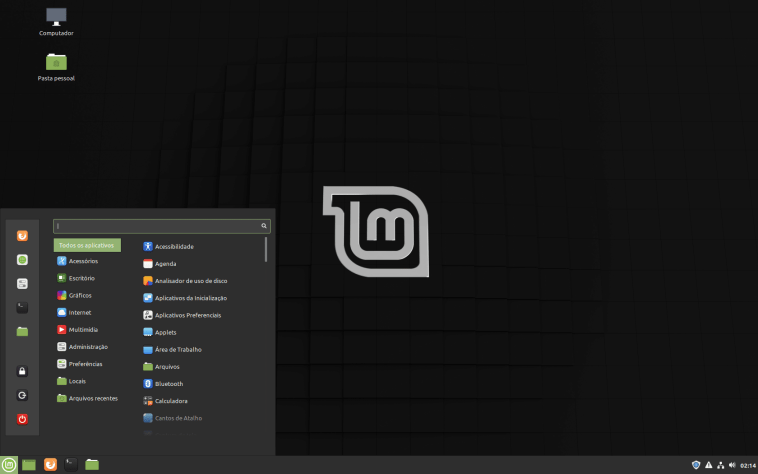
\includegraphics[width=\textwidth]{include/menu.png}\newline
			\caption{Le Menu}
			\label{fig:menu}
		\end{figure}\par
		Le menu démarrer permet d'accéder à l'ensemble des applications qui sont présentes sur votre ordinateur.
		Comme il est ordonné, il est très simple de s'y retrouver et de l'utiliser.
		Ce menu vous sera indispensable lorsque vous aurez besoin d'un logiciel ou autre.\par
		Le menu démarrer se décompose en quatre parties :
		\begin{itemize}
			\item La barre latérale tout à gauche contient lesz outils de bases : le Navigateur Firefox (voir Sections \ref{sec:descfirefox} et \ref{sec:utiliserfirefox}); l'invit de commande (voir Section \ref{sec:utiliserterminal}); ...;
			\item Le menu principal au centre contient toutes les catégories de logiciel;
			\item Le menu de droite contient les éléments contenu dans la catégorie sélectionnée;
			\item La barre de recherche en haut permet de rechercher par mots-clés;
		\end{itemize}
	\subsection{Le gestionnaire de fichiers}\label{sec:fichiers}
		Le gestionnaire de fichiers vous permet de ranger et de retrouver facilement vos répertoires et vos fichiers divers.
		\begin{figure}[h]
			\centering
			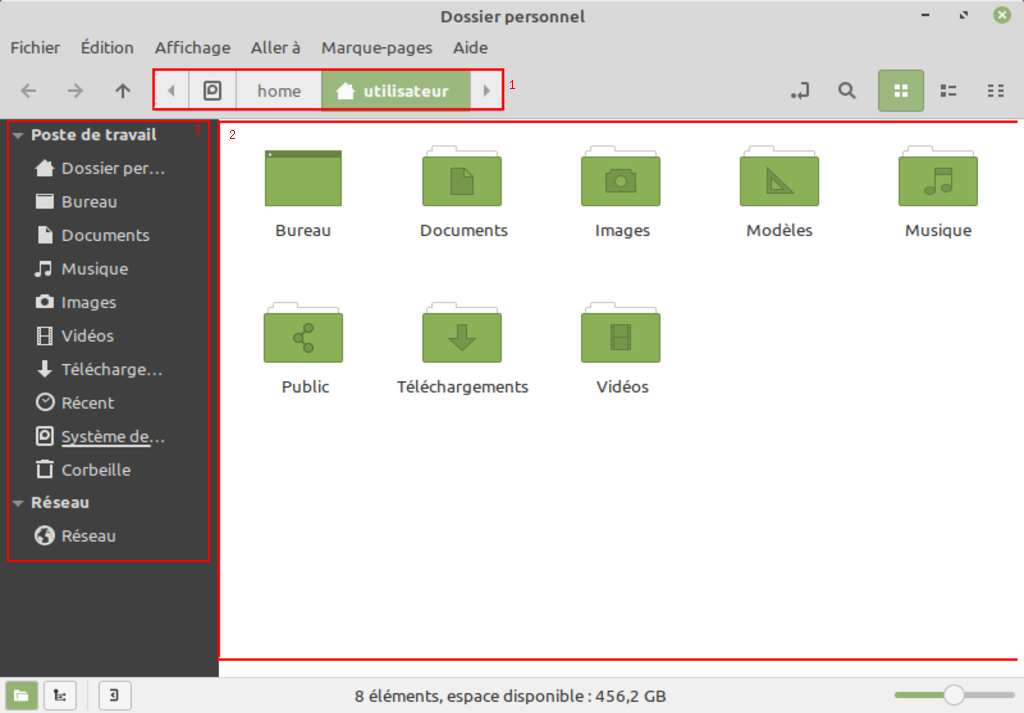
\includegraphics[width=\textwidth]{include/fichiers.png}
			\caption{Le gestionnaire de fichiers}
			\label{fig:fichiers}
		\end{figure}\par
		Le gestionnaire de fichiers se trouve sur la barre des tâches (voir la Section \ref{sec:barretaches}).
		Il se trouve également dans le Menu (voir la Section \ref{sec:menu}), sur la barre latérale gauche.
		Il s'agit de l'icône qui est représenté par un petit dossier vert.\par
		La fenêtre qui s'ouvre vous permet d'accéder à tous les documents que vous avez enregistrés sur votre ordinateur mais aussi sur vos disques amovibles (par exemple une clé USB).
		\begin{enumerate}
			\item Chemin du répertoire courant (le répertoire que vous consultez);
			\item Ensemble des répertoires et des fichiers du répertoire courant;
			\item Accès rapide aux répertoires fréquemment utilisés
			\begin{itemize}
				\item La partie \texttt{Poste de travail} affiche l'ensemble des repertoires enregistrer sur votre disque dur interne;
				\item La partie \texttt{Réseau} affiche les répertoires partagés sur un même réseau local;
				\item La partie \texttt{Périphériques} peut apparaitre lorsque un (ou plusieurs) disque(s) amovible(s) est inséré dans votre ordinateur. Le repertoire du disque apparait dans cette partie.
			\end{itemize}
		\end{enumerate}
	\subsection{Extinction de l'ordinateur}
		Lorsque vous avez terminé d'utiliser l'ordinateur, il faut l'éteindre. Eteindre son équipement après chaque utilisation est important. 
		Cela permet notamment de réduire la chaleur des composants, de résoudre certains bugs liés à une trop longue utilisation, de limiter sa consommation énergétique, etc.\par
		Pour éteindre votre machine :
		\begin{enumerate}
			\item Ouvrez le Menu et cliquez sur l'icône rouge en bas à gauche de la barre latérale;
			\item Une boîte de dialogue s'ouvre et vous propose plusieurs options;
			\item Cliquez sur celle toute à droite "\texttt{Eteindre}" (le bouton rouge);
			\begin{figure}[h]
				\centering
				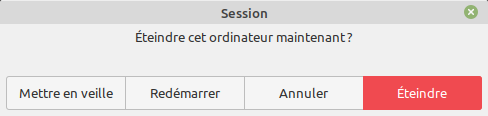
\includegraphics[width=.8\textwidth]{include/eteindre.png}
				\caption{Eteindre son ordinateur}
				\label{fig:eteindre}
			\end{figure}
			\item Vorte ordinateur affiche le logo de Linux Mint puis s'éteint.
		\end{enumerate}
		Comme vous pouvez le voir sur la figure \ref{fig:eteindre}, vous pouvez également "\texttt{Mettre en vielle}" (votre ordinateur est toujours allumé mais consomme moins d'énergie et mets les applications en pause) ou "\texttt{Redémarrer}" (l'ordinateur arrête tous les programmes et se relance) votre ordinateur.
		Mettre en veille son ordinateur peut être utile lorsque que vous prenez une pause mais que vous ne voulez pas tout arrêter par exemple.
		Redémarrer son ordinateur peut être utile lorsque celui-ci commence à ralentir ou boguer.
		Cela peut aussi être nécessaire après l'installation d'un nouveau logiciel ou d'une mise à jour.
\section{Utilisation d'un périphérique amovible}
	Un périphérique amovible est un accessoire connecté à l'ordinateur qui vient le compléter.
	Cela peut être, un clavier, une souris, une clé USB, une imprimante, etc.\par
	La plupart du temps, votre ordinateur reconnaît automatiquement votre périphérique.
	C'est le cas pour la plupart des clé USB de stockage ainsi que des disques durs externes.
	Pour d'autres accessoires commes une imprimante ou un scanner, il faut parfois installer le pilote manuellement.
	Lorsque vous brancher votre accessoire, une notification peut apparaitre en haut à droite de l'écran pour vous signifier qu'un nouveau périphérique a bien été détecté.
	S'il s'agit d'un périphérique de stockage (clé USB, disque dur externe...) une fenêtre s'ouvre automatiquement dans le répertoire du périphérique.
	S'il s'agit d'un autre périphérique, la notification peut vous indiquer qu'il faut installer le pilote adéquat.
	Cliquez sur cette notification et faites la recherche de nouveaux pilotes si cela est nécessaire.
	Installer les pilotes indiqués.
	Une fois cela fait, votre ordinateur aura peut-être besoin de redémarrer.
	Puis vous pourrez utiliser votre périphérique.
\section{Paramètrage du compte}
	Pour personnaliser d'avantage votre ordinateur vous pouvez modifier le nom d'utilisateur, le mot de passe, l'avatar, le thème général...
	Dans cette section, nous expliquons comment faire ces petits changements.
	\subsection{Modifier le nom de l'utilisateur}
		Le nom d'utilisateur est le nom que vous donner au compte enregistré sur votre ordinateur.
		Vous pouvez le personnalier, pour cela :
		\begin{enumerate}
			\item Ouvrez le Menu;
			\item Cliquez sur "Administration" puis descendez et cliquez sur "Utilisateurs et Groupes";
			\item Si besoin, entrez votre mot de passe;
			\item Cliquez sur votre compte (ici "utilisateur");
			\begin{figure}[h]
				\centering
				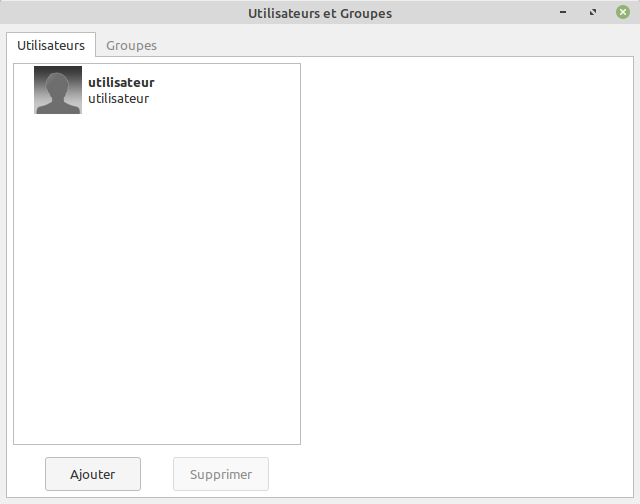
\includegraphics[width=\textwidth]{include/users.png}
				\caption{Liste des utilisateurs}
				\label{fig:nomuser}
			\end{figure}
			\item Cliquez sur le nom d'utilisateur actuel face au champs "Nom :"
			\begin{figure}[h]
				\centering
				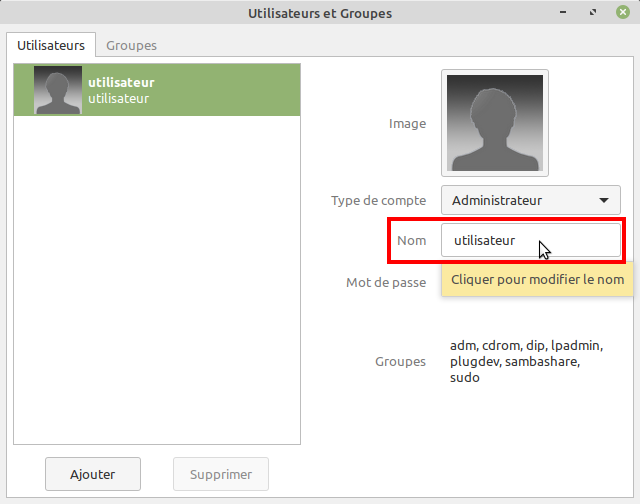
\includegraphics[width=\textwidth]{include/nomuser.png}
				\caption{Modifier le nom utilisateur}
				\label{fig:nomuser}
			\end{figure}
			\item Tapez votre nouveau nom d'utilisateur puis appuyez sur la touche "\texttt{Entrée}".
		\end{enumerate}
		Félicitations ! Vous avez changé votre nom utilisateur.
	\subsection{Modifier le mot de passe}
		Le mot de passe de votre ordinateur est très important. 
		Il protège votre ordinateur contre une utilisation malvaillante ou d'une erreur de manipulation en vous demandant de confirmer votre mot de passe.
		Vous pouvez le modifier, pour cela :
		\begin{enumerate}
			\item Ouvrez le Menu;
			\item Cliquez sur "Administration" puis descendez et cliquez sur "Utilisateurs et Groupes";
			\item Si besoin, entrez votre mot de passe;
			\item Cliquez sur votre compte (ici "utilisateur");
			\begin{figure}[h]
				\centering
				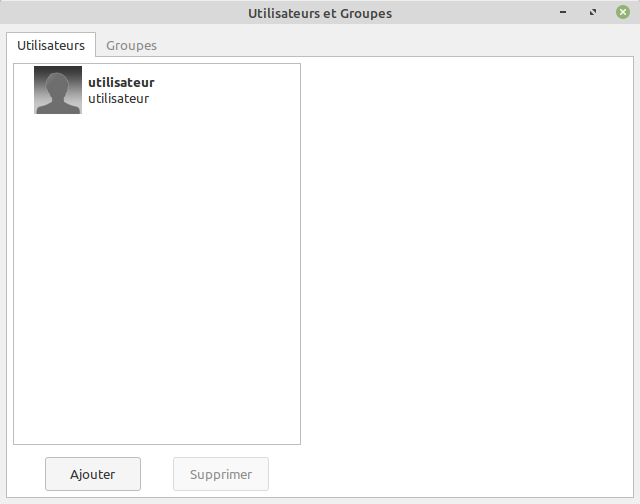
\includegraphics[width=\textwidth]{include/users.png}
				\caption{Liste des utilisateurs}
				\label{fig:nomuser}
			\end{figure}
			\item Cliquez sur le mot de passe caché actuel face au champs "Mot de passe :"
			\begin{figure}[h]
				\centering
				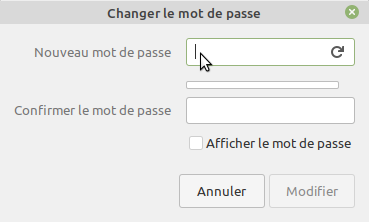
\includegraphics[width=.5\textwidth]{include/mdpuser.png}
				\caption{Modifier le mot de passe}
				\label{fig:nomuser}
			\end{figure}
			\item Tapez votre nouveau mot de passe et confirmez-le.
		\end{enumerate}
		Félicitations ! Vous avez changé votre mot de passe.
	\subsection{Modifier l'avatar}
		L'avatar de votre compte est visible lors de votre connexion à l'ordinateur et lors de l'affichage de votre compte.
		Vous pouvez le personnaliser, pour cela :
		\begin{enumerate}
			\item Ouvrez le Menu;
			\item Cliquez sur "Administration" puis descendez et cliquez sur "Utilisateurs et Groupes";
			\item Si besoin, entrez votre mot de passe;
			\item Cliquez sur votre compte (ici "utilisateur");
			\begin{figure}[h]
				\centering
				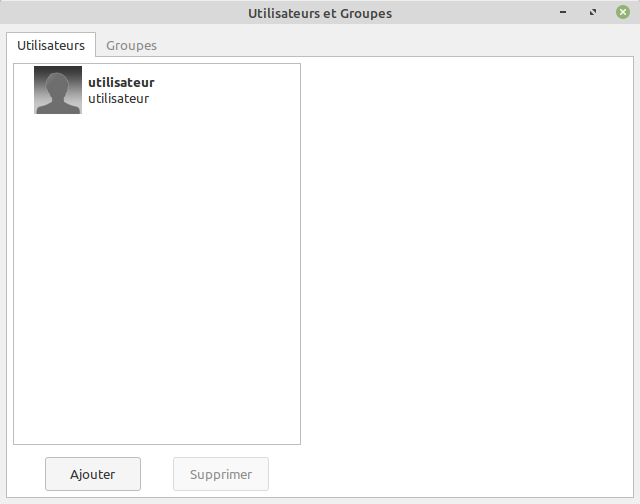
\includegraphics[width=\textwidth]{include/users.png}
				\caption{Liste des utilisateurs}
				\label{fig:mdpuser}
			\end{figure}
			\item Cliquez sur le mot de passe caché actuel face au champs "Mot de passe :"
			\begin{figure}[h]
				\centering
				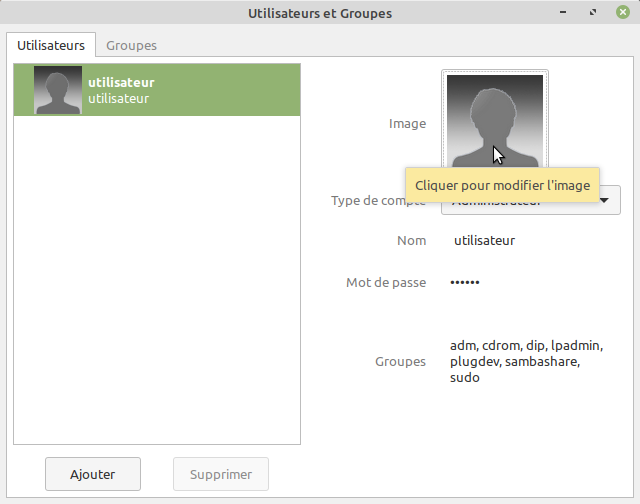
\includegraphics[width=\textwidth]{include/avataruser.png}
				\caption{Modifier l'avatar du compte}
				\label{fig:avataruser}
			\end{figure}
			\item Sélectionnez un nouvel avatar.
		\end{enumerate}
		Félicitations ! Vous avez changé votre avatar.
	\subsection{Modifier le thème}\label{sec:theme}
		 Pour personnaliser un peu plus votre environnement de travail ou pour un meilleur confort visuel, vous aurez peut-être envie de changer le thème de votre ordinateur.
		 Pour cela, rien de plus simple :
		 \begin{enumerate}
		 	\item Ouvez le Menu;
		 	\item Cliquez sur "\texttt{Préférences}" puis descendez jusqu'à "\texttt{Thèmes}";
		 	\item 
		 	\begin{figure}[h]
		 		\centering
		 		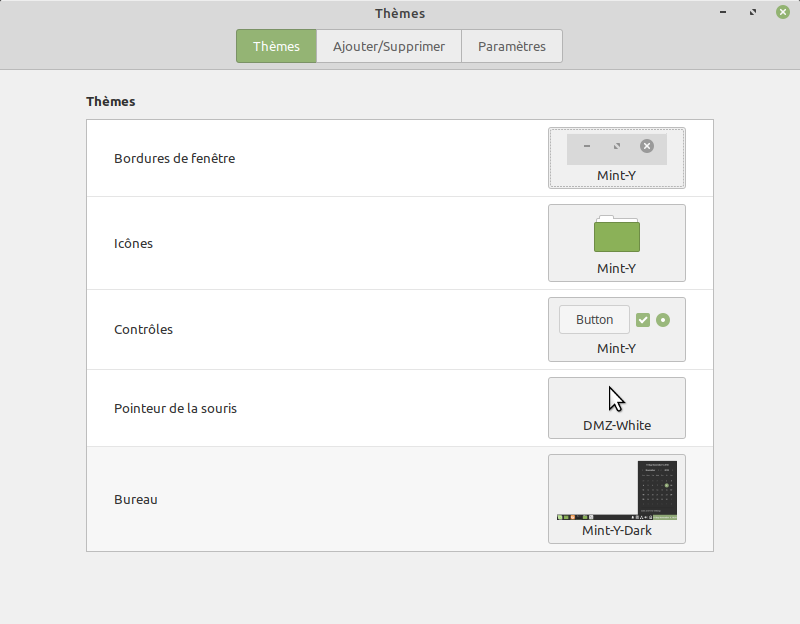
\includegraphics[width=.8\textwidth]{include/themes.png}
		 		\caption{Paramétrage du thème de l'ordinateur}
		 		\label{fig:themes}
		 	\end{figure}
		 	Une nouvelle fenêtre s'ouvre avec les champs suivants :
		 	\begin{itemize}
		 		\item \texttt{Bordure de fenêtre} : modifier la couleur d'une fenêtre;
		 		\item \texttt{Icônes} : modifier l'aspect et la couleur des icônes répertoire;
		 		\item \texttt{Contrôles} : modifier l'aspect et la couleurs des boutons d'une fenêtre;
		 		\item \texttt{Pointeur de la souris} : modifier la couleur du pointeur de la souris;
		 		\item \texttt{Bureau} : modifier l'aspect et la couleur de la barre de tâches et du menu.
		 	\end{itemize}
		 \end{enumerate}

\chapter{Logiciels et applications}\label{sec:logiciels}
Sous Linux Mint, l'installation de logiciels et d'applications se fait uniquement via un portail particulier -la Logithèque- ou par lignes de commande.
La Logithèqe est le portail qui vous permet de rechercher et d'installer des applications et des logiciels directement sur votre ordinateur.\par
Dans ce chapitre, nous expliquons comment utiliser la logithèque.
Nous détaillons également quelques logiciels libres indispensables pour bien démarrer votre expérience numérique.
Seuls quelques logiciels seront détaillés dans ce chapitre, nous vous invitons à explorer la logithèque ou de consulter des sites tels que \href{https://framalibre.org/}{https://framalibre.org/} (dernière consultation le 31/03/2021) qui pourront vous inspirer et vous aider à trouver le logiciel libre de vos rêves.
\section{La Logithèque de Linux Mint}\label{sec:logitheque}
	La Logithèque présente sur votre ordinateur se présente comme une immense bibliothèques d'applications.
	Elle sera votre meilleure alliée pour rechercher et explorer rapidement et très simplement de nouveau logiciels à intégrer à votre ordinateur.\par
	Pour accéder à la Logithèque :
	\begin{enumerate}
		\item Ouvrez le Menu;
		\item Cliquez sur la section "\texttt{Administration}" puis descendez jusqu'à "\texttt{Logithèque}".
	\end{enumerate}\par
	\begin{figure}[h]
		\centering
		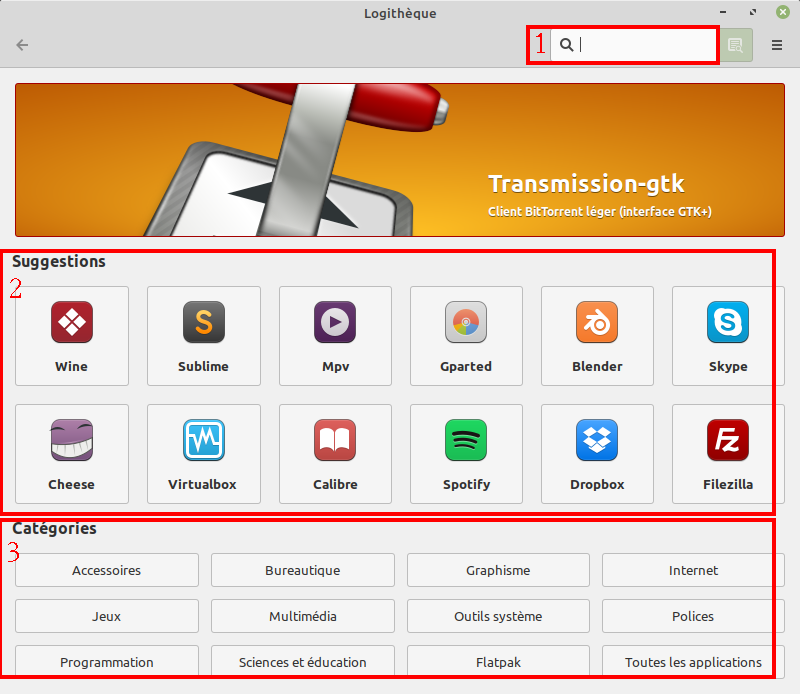
\includegraphics[width=.8\textwidth]{include/logitheque.png}
		\caption{Accueil de la Logithèque}
		\label{fig:logitheque}
	\end{figure}\par
	Une fois sur l'écran d'accueil, vous pouvez rechercher un logiciel de différentes manières :
	\begin{enumerate}
		\item Tapez dans la barre de recherche placée en haut à droite de la fenêtre si vous connaissez le nom du logiciel que vous chercher ou vous souhaitez effectuer une recherche par mots-clé;
		\item Découvrez un logiciel suggéré par page d'accueil;
		\item Cherchez sur la catégorie que vous souhaitez explorer.
	\end{enumerate}
	\subsection{Un exemple de recherche dans la logithèque}\label{sec:exlogitheque}
		Voici un petit exemple simple pour rechercher et installer facilement un logiciel ou une application via la logithèque.\par
		Pour cela, nous allons prendre l'exemple d'une application nous permettant d'obtenir la météo.\par
		Une fois sur l'écran d'accueil de la Logithèque, nous tapons "\textit{météo}" dans la barre de recherche située en haut à droite de la fenêtre puis nous appuyons sur la touche "\texttt{Entrée}".
%		\begin{figure}[h]
%			\centering
%			\includegraphics[width=.8\textwidth]{include/meteo1.png}
%			\caption{Recherche du mot-clé "\textit{météo}" dans la barre de recherche de la logithèque}
%			\label{fig:meteo1}
%		\end{figure}\par
		Une liste d'applications s'affiche alors. 
		Nous en choisissons une parmi cette liste et cliquons dessus.
%		\begin{figure}
%		\includegraphcis[width=.8\textwidth]{include/meteo2.png}
%		\caption{Liste de résultat pour la recherche "\textit{météo}"}
%		\label{fig:meteo2}
%		\end{figure}\par
		Le détail pour cette application s'affiche.
		On y retrouve une description, des captures d'écrans et les avis d'autres utilisateurs.
		Nous cliquons sur "\texttt{Installation}"
		\textit{faire une subfigure avec meteo4 et meteo5}
\section{Les logiciels indispensables pour bien démarrer}
Savoir télécharger des logiciels sur son ordinateur, c'est bien.
Savoir quels logiciels installer, c'est mieux !\par
Dans cette partie, nous présentons quelques logiciels simple et indispensables.
Bien d'autres logiciels seront utiles en plus de ceux présentez ici.
N'hésitez pas à explorer la logithèque.
	\subsection{Le pack LibreOffice}\label{sec:libreoffice}
		\begin{minipage}[c]{0.3\textwidth}
			\centering
			
\includegraphics[width=\textwidth]{include/lo_logo.png}
		\end{minipage}
		\begin{minipage}[c]{.7\textwidth}
			Le pack LibreOffice est indispensable lorsque l'on souhaite rédiger des documents de toute sorte.
			Il s'agit d'une "suite bureautique", c'est-à-dire d'un ensemble de logiciels vous permettant de réaliser différentes tâches de bureau.
			Grâce à une suite bureautique, vous pouvez lire et rédiger des documents, des feuilles de calculs, des diaporamas, etc.
		\end{minipage}\par
			La suite bureautique LibreOffice es très puissante et très simple à utiliser.
			Elle est composée des fonctionnalités suivantes :
		\begin{itemize}
			\item LibreOffice writer vous permet de rédiger des documents textes et de les mettre en forme.
			Ces documents sont au format .odt. 
			Il est aussi possible d'imprimer ses documents ou de les exporter au format .pdf via LibreOffice Writer.
			\item LibreOffice Calc vous permet de créer et d'utiliser des classeurs.
			Ces documents sont au format .ods. 
			Ils sont très utilisés pour faire des feuilles de calculs, enregistrer des données, etc.
			\item LibreOffice Impress vous permet de créer des diaporamas. 
			Ces documents sont au format .odp.
			LibreOffice Impress vous sera très utile pour préparer des supports visuels, des diaporamas pour des exposés, des réunions, etc.
			Il vous sera possible d'exporter votre document au format .pdf.
			\item LibreOffice Draw vous permet de faire toute sorte de dessins.
			Ces documents sont au format .odg.
			Très pratique pour faire un petit dessin rapide, un schéma plus complexe ou bien encore un support visuel.
			\item LibreOffice Math vous permet de rédiger des formules mathématiques.
			Ces documents sont au format .odf;
			Cet outil vous permet de prnedre en notes des formules mathématiquesdiverses, d'utiliser des opérateurs (unitaires, binaires, logiques...), des relations, de rédiger des matrices, d'utiliser des symboles, etc.
			\item LibreOffice Base vous permet de créer et de gérer une base de données relationnelles.
			Il est possible de créer une nouvelle base ou bien de se connecter à une base (JDBC par exemple). 
		\end{itemize}\par
		La suite bureautique de LibreOffice vous permet donc de lire et de rédiger des fichiers sous des formats de documents dits ouverts (.odf) mais aussi les formats de la suite bureautique de Microsoft (.docx, xlsx...).\par
		Pour en savoir plus sur le pack LibreOffice et sur ses nombreuses fonctionnalités, vous pouvez consulter le site officiel \footnote{
		\href{https://fr.libreoffice.org}{https://fr.libreoffice.org} \textit{(dernière consultation le 02/04/2021)}}.
	\subsection{Mozilla Firefox}\label{sec:descfirefox}
		\begin{minipage}[c]{.7\textwidth}
			Mozilla Firefox ext un navigateur web.
			C'est-à-dire que son rôle est d'afficher des pages web (par exemple des pages au format .html ou .php).
			Comme son nom l'indique, un navigateur vous permet de "naviguer" entre différentes pages web via des liens.
			Mozilla Firefox est très connu et très utilisé à travers le monde.
			Il vous offre beaucoup de paramètres d'affichages, de langues mais aussi de sécurité.
			C'est également un navigateur libre.
		\end{minipage}
		\begin{minipage}[c]{.3\textwidth}
			\centering
			
\includegraphics[width=\textwidth]{include/mf_logo.jpg}
		\end{minipage}\par
		Pour un navigateur web, cela garanti notamment une certaine sécurité sur nos données personnelles.
		En effet, Firefox n'a aucun intérêt à revendre les données de ces utilisateurs, donc les données collectées ne servent qu'au bon fonctionnement du logiciel.
		Ce navigateur permet également de bloquer les traqueurs publicitaires.\par
		N'hésitez pas à consulter le site officiel de Mozilla Firefox\footnote{\href{https://www.mozilla.org/fr/firefox/features/}{https://www.mozilla.org/fr/firefox/features/} (dernière consultation le 06/04/2021)} pour plus d'informations.
		Vous pouvez aussi consulter la liste des extensions\footnote{\href{https://addons.mozilla.org/fr/firefox/}{https://addons.mozilla.org/fr/firefox/} (dernière consultation le 06/04/20201)} proposées par Mozilla Firefox.
		Les extensions (ou plugins) sont des "petits plus" qu'on ajoute au navigateur pour l'améliorer et pour obtenir une fonctionnalité bien particulière.

\chapter{Internet}
Maintenant que nous nous sommes familiarisés avec cet environnement, il est temps d'aller surfer sur le web.
Internet, c'est la porte ouverte d'une connaissance mondiale partagée.
S'il permet d'accéder à une multitude d'informations et de contenus divers, il est important de rappeler qu'Internet est aussi un endroit où des personnes malvaillantes peuvent se trouver.
Elles peuvent propager de fausses informations (fake news en anglais), recourir à des virus ou à des logiciels malvaillants pour entrer dans votre ordinateur, etc.
Du contenu se trouvant sur Internet peut aussi ne pas convenir aux enfants.
Il faut donc s'en protéger et adopter les bons gestes lorsque l'on utilise internet et garder un esprit critique face à ce qu'on peut y trouver\par
Dans ce chapitre consacré à Internet, nous verrons dans un premier temps comment nous connecter à Internet.
Dans un deuxième temps, nous étudirons le navigateur Mozilla Firefox qui sera notre "porte" pour aller sur le web.
Dans un troisième temps, nous allons voir comment utiliser le moteur de recherche Lilo qui nous permettra de faire nos premières recherches sur internet.
Enfin, nous aborderons la question de la sécurité sur Internet.
\section{Se connecter à son réseau}
	Avant toute chose, nous devons être connecté à Internet. 
	C'est-à-dire que nous devons établir un lien entre l'ordinateur et le réseau.
	Pour cela, deux façons de procéder :
	\begin{enumerate}
		\item en se connectant via un un câble reliant l'ordinateur à la box ;
		\item en se connectant via un le WiFi.
	\end{enumerate}
	\subsection{Avec un câble éthernet}
		Pour connecter votre ordinateur, vous devez utiliser un câble RJ45 (éthernet).
		L'embout ressemble à ceci :
		\begin{figure}[h]
			\centering
			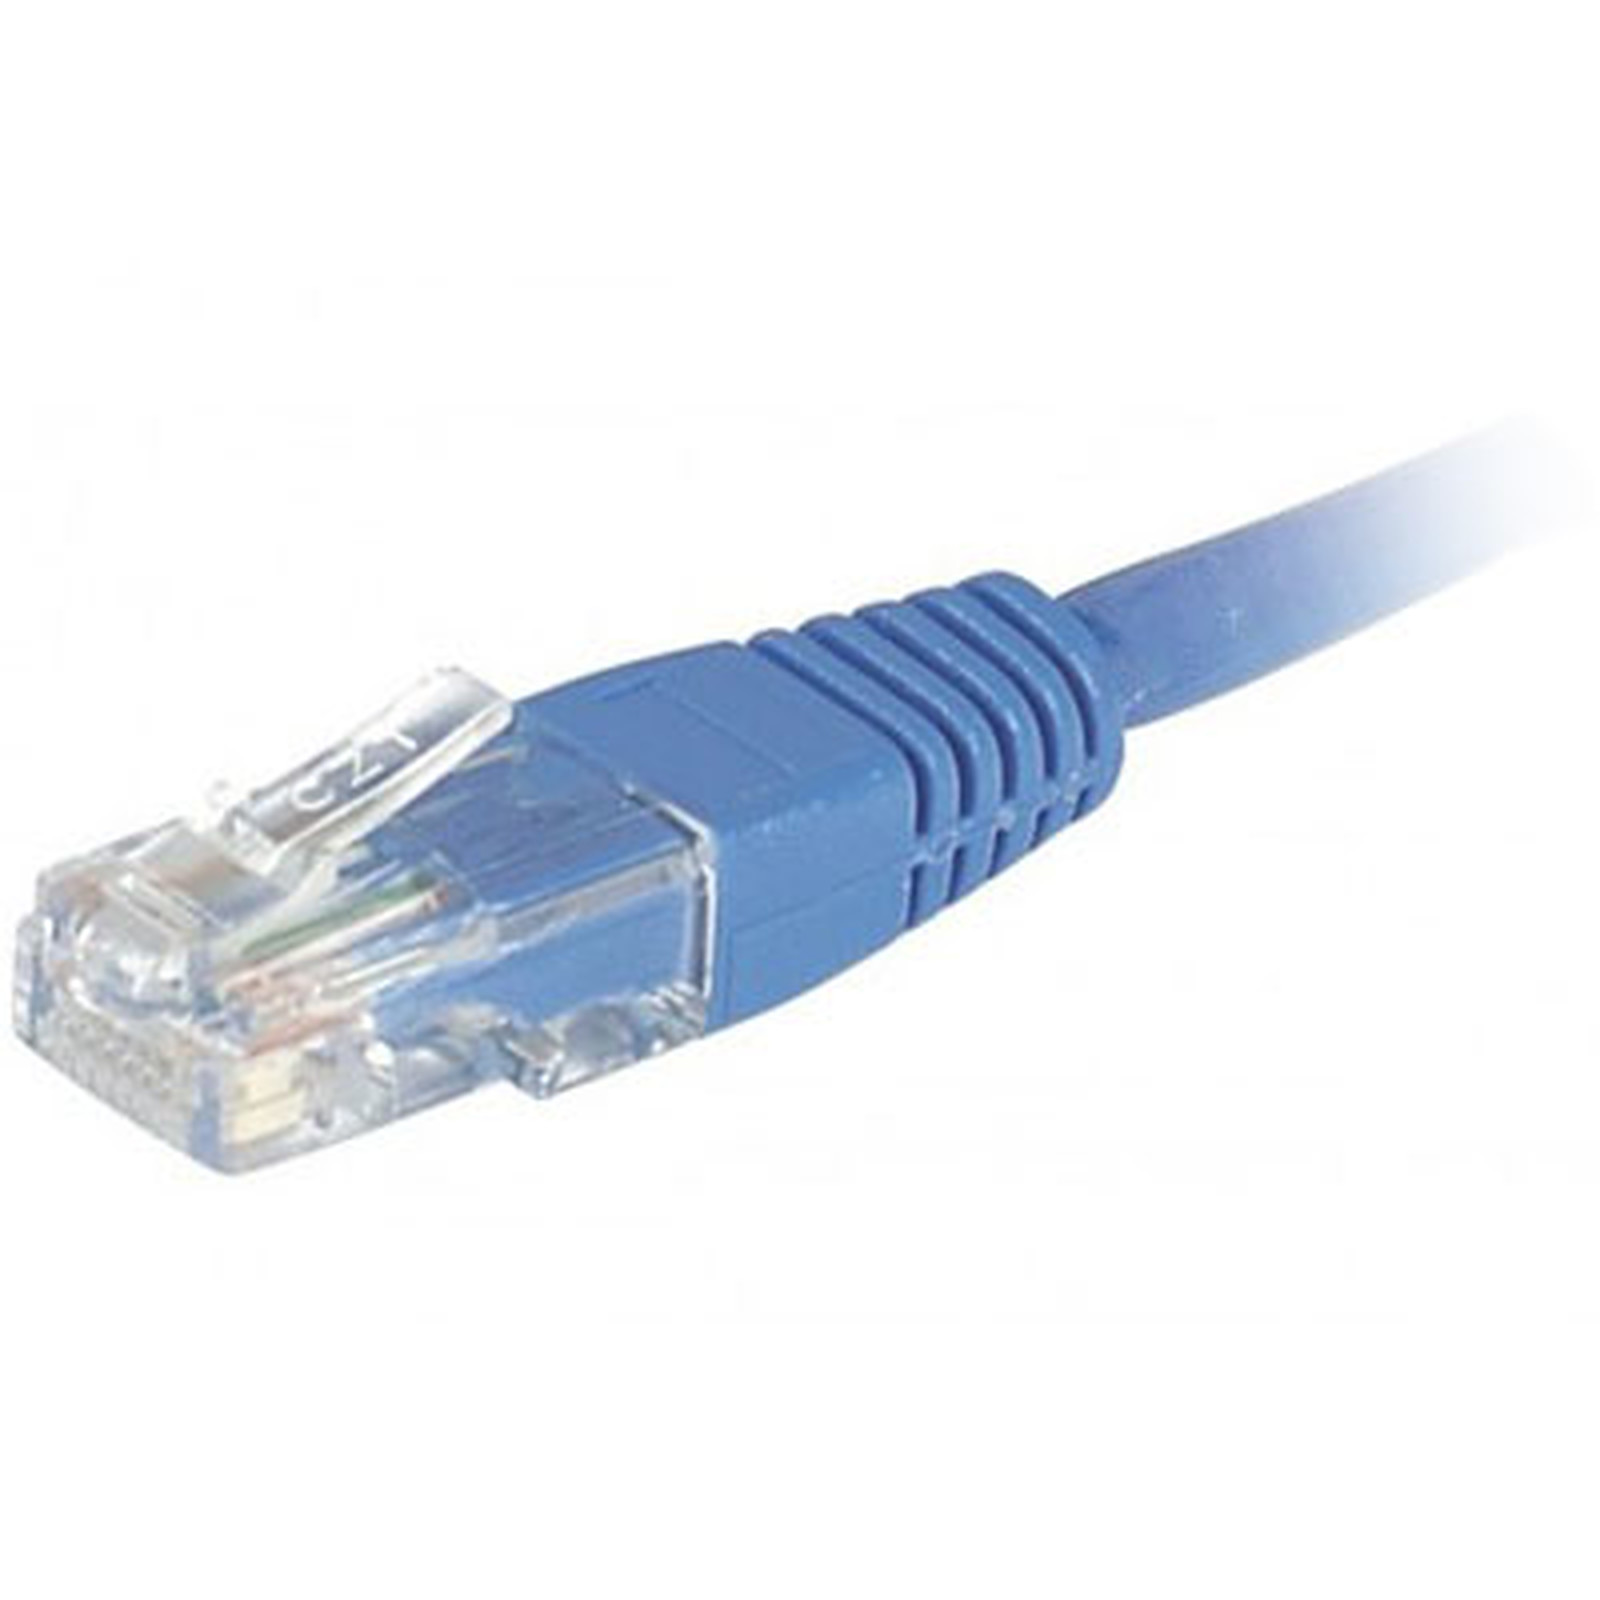
\includegraphics[scale=0.05]{include/rj45.jpg}
			\label{fig:rj45}
			\caption{Câble éthernet RJ45}
		\end{figure}\par
		Utiliser ce câble en le branchant d'un côté à votre ordinateur et de l'autre à votre box (ou dans la prise éthernet de votre mur si elle existe).
		Une fois branché des deux côtés, l'icône "Internet" à droite sur la barre des tâches doit avoir changé et ressembler à ceci :
		\begin{figure}[h]
		\begin{subfigure}{\textwidth}
			\centering
			
\includegraphics[width=\textwidth]{include/connexion_barre.png}
			\caption{Icône indicant l'état de connexion sur la barre des tâches}
			\label{fig:barre_taches_connexion}
		\end{subfigure}\newline
		\begin{subfigure}{.5\textwidth}
		  \centering
		  
\includegraphics{include/non_connect.png}
		  \caption{Avant le branchement du \newline câble RJ45}
		  \label{fig:non_connect_rj45}
		\end{subfigure}
		\begin{subfigure}{.5\textwidth}
		  \centering
		  
\includegraphics{include/connect.png}
		  \caption{Après le branchement du \newline câble RJ45}
		  \label{fig:connect_rj45}
		\end{subfigure}
		\caption{Affichage de l'état de connexion avec un câble éthernet}
		\label{fig:connexion_rj45}
		\end{figure}\par
		Une notification a pu aussi apparaître tout en haut à droite de votre écran.
		Elle doit ressember à ceci :
		\begin{figure}[h]
			\centering
			\begin{subfigure}{.49\textwidth}
				\centering
				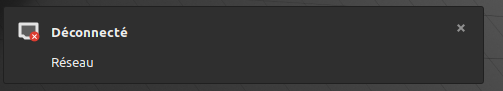
\includegraphics[width=\textwidth]{include/notif_deco.png}
				\caption{Notification "ordinateur déconnecté" d'Internet}
				\label{fig:notif_deco_rj45}
			\end{subfigure}
			\begin{subfigure}{.5\textwidth}
				\centering
				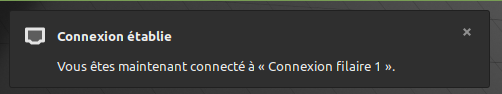
\includegraphics[width=\textwidth]{include/notif_co.png}
				\caption{Notification "ordinateur connecté" à Internet}
				\label{fig:notif_co_rj45}
			\end{subfigure}
			\label{fig:notif_connexion_rj45}
			\caption{Notifications de connexion au réseau Internet}
		\end{figure}\par
		Vous voilà maintenant connecter à Internet !
	\subsection{Avec le WiFi}
		Avant de commencer, si vous disposez d'un ordinateur portable, votre ordinateur dispose probablement d'un système de connexion au WiFi intégré et vous pouvez directement essayer de vous connecter.
		Si vous disposez d'un ordinateur de bureau, vous aurez probablement besoin d'un dispositif de connexion WiFi externe.
		Nous vous conseillons d'utiliser une clé USB WiFi.
		Elles sont très simple d'utilisation.
		Pour la plupart de ces clés WiFi, il suffit de les brancher dans l'ordinateur et vous pourrez vous connecter aux réseaux WiFi.
		\begin{figure}[h]
			\centering
			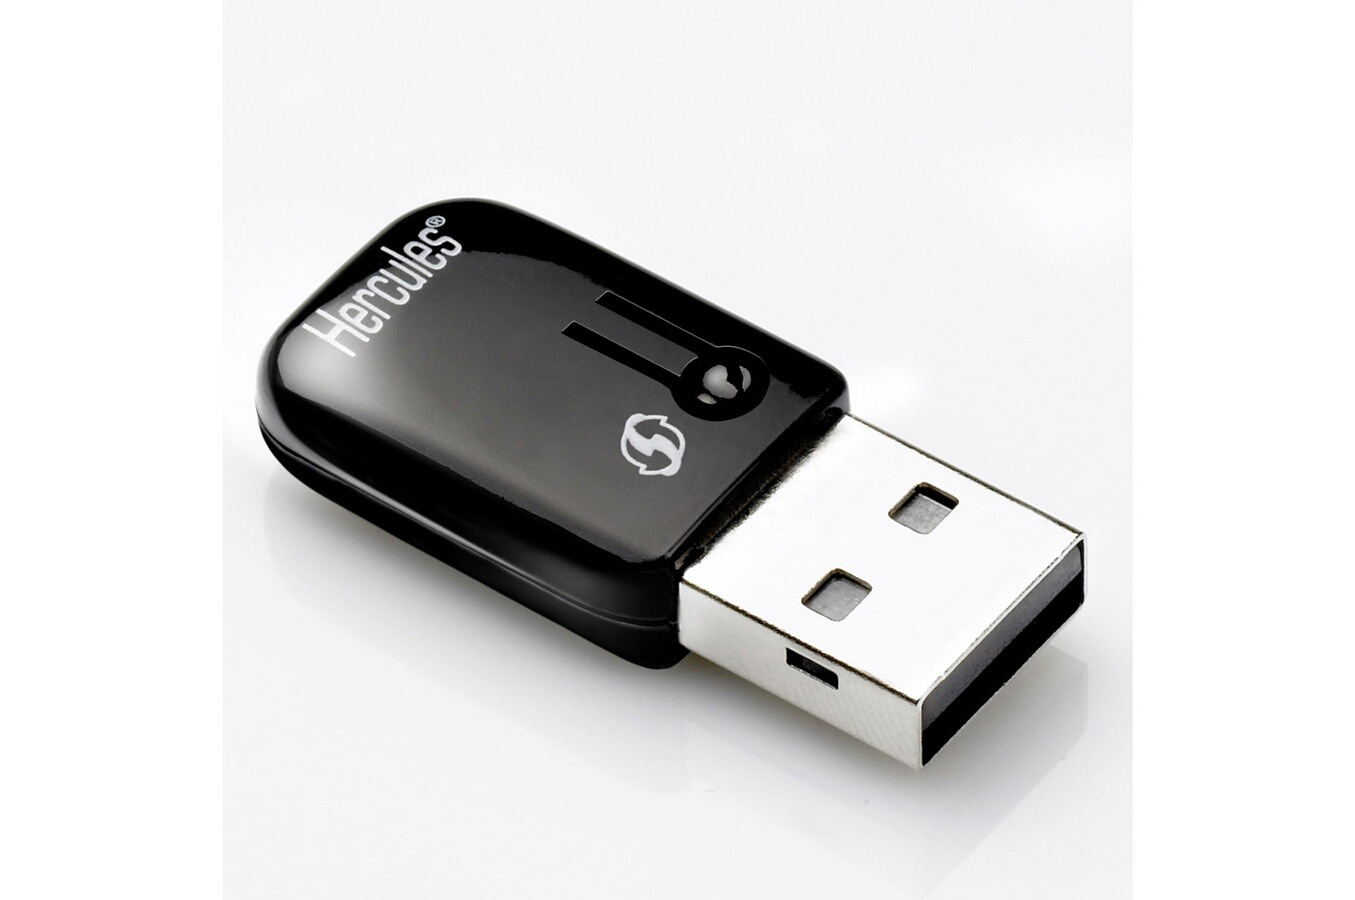
\includegraphics[width=.4\textwidth]{include/clewifi.jpg}
			\caption{Exemple d'une clé USB WiFi}
			\label{fig:clewifi}
		\end{figure}\par
		Pour vous connecter, cliquez sur l'icône indiquant l'état de connexion de votre ordinateur. Cette icône se situe à droite sur la barre des tâches.
		\begin{figure}[h]
			\centering
			
\includegraphics[width=\textwidth]{include/connexion_barre.png}
			\caption{Icône indicant l'état de connexion sur la barre des tâches}
			\label{fig:barre_connexion}
		\end{figure}\par
		Un petit menu s'affiche alors.
		Vérifier que le bouton face à "Wi-Fi" est bien en position marche.
		Cliquez sur le réseau WiFi qui vous intéresse.
		Une boîte de dialogue s'ouvre pour vous demander un mot de passe.
		Entrer le mot de passe de votre réseau et cliquez sur "Se conecter".
		\begin{figure}[h]
			\centering
			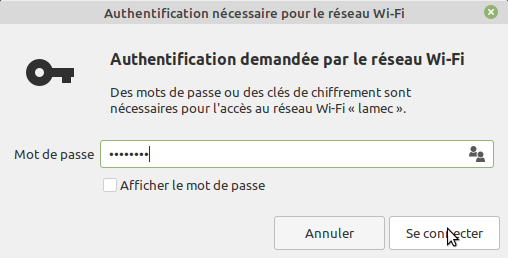
\includegraphics[width=.9\textwidth]{include/wifi_mdp.png}
			\caption{Boîte de dialogue de connexion à un réseau WiFi}
			\label{fig:connexion_wifi}
		\end{figure}
		Si le mot de passe est incorrect, alors la boîte de dialogue vous demandera à nouveau d'entrer le mot de passe.\par
		La boîte de dialogue disparait et l'icône "Internet" à droite sur la barre des tâches doit avoir changé et ressembler à ceci :
		\begin{figure}[h]
			\centering
			
\includegraphics{include/connect_wifi.png}
			\label{fig:iconeconnecte}
			\caption{Icône WiFi "connecté"}
		\end{figure}
		\newline
		Une notification a pu aussi apparaître tout en haut à droite de votre écran.
		Elle doit ressember à ceci :
		\begin{figure}[h]
		\centering
			\begin{subfigure}{.51\textwidth}
				\centering
				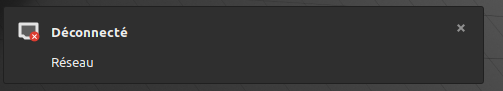
\includegraphics[width=\textwidth]{include/notif_deco.png}
				\caption{Notification "ordinateur déconnecté" d'Internet}
				\label{fig:notif_deco_wifi}
			\end{subfigure}
			\begin{subfigure}{.48\textwidth}
				\centering
				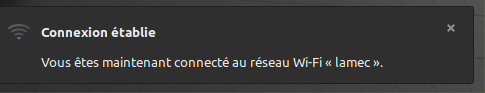
\includegraphics[width=\textwidth]{include/notif_wifi.png}
				\caption{Notification "ordinateur connecté" à Internet}
				\label{fig:notif_co_wifi}
			\end{subfigure}
			\caption{Notifications de connexion à un réseau WiFi}
			\label{fig:notif_wifi}
		\end{figure}\par
		Félicitations, vous êtes connecté à Internet !
\section{Utiliser le navigateur Mozilla Firefox}\label{sec:utiliserfirefox}
	Nous avons vu dans la Section \ref{sec:deffirefox} de nombreuses informations relatives à ce navigateur libre.
	Si ce n'est pas déjà fait, nous vous encourageons à lire cette section pour prendre connaissance des fonctionnalités présentées par Firefox.\par
	Ici, nous allons voir comment utiliser le navigateur Mozilla Firefox.\par
	Pour commencer, ouvrez le navigateur web.
	Pour cela, vous pouvez cliquez sur l'icône "Firefox" qui se trouve sur votre barre des tâche à droite de l'îcône du menu démarrer .
	\begin{figure}[h]
		\centering
		
\includegraphics[width=\textwidth]{include/mf_barre.png}
		\caption{Localisation du navigateur web Mozilla Firefox sur la barre des tâches}
		\label{fig:mf_barre}
	\end{figure}\par
	Une nouvelle fenêtre s'ouvre et affiche votre page d'accueil.
	Ici, notre page d'accueil est le moteur de recherche Lilo (voir la Section \ref{sec:ilo}).
	\begin{figure}[h]
		\centering
		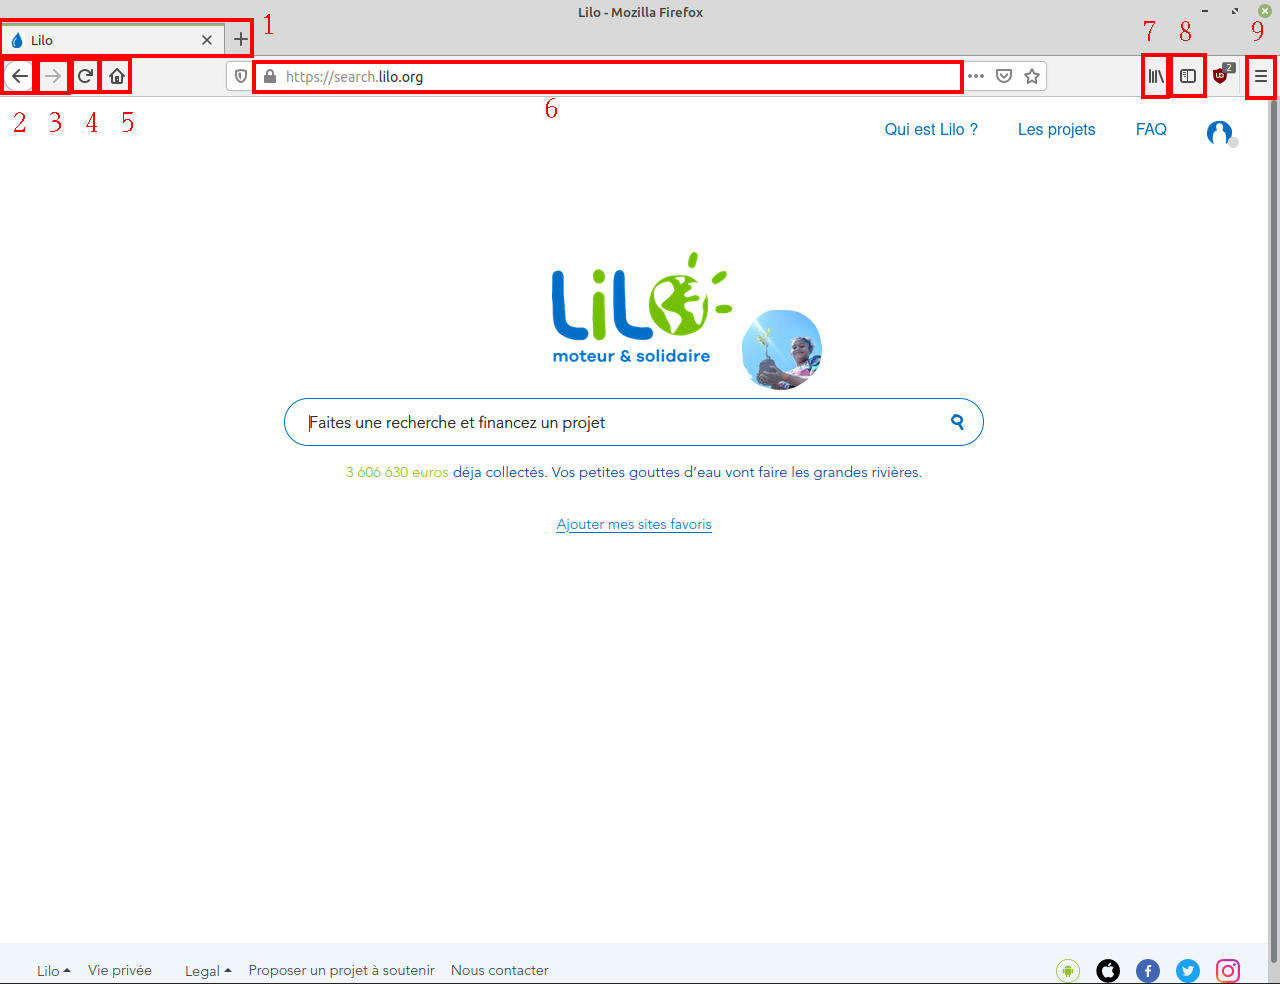
\includegraphics[width=.9\textwidth]{include/accueil_mf.png}
		\caption{Ouverture de Mozilla Firefox}
		\label{fig:accueil_mf}
	\end{figure}
	\begin{enumerate}
		\item Les onglets.\newline
				Vous pouvez ouvrir plusieurs pages dans une seule fênetre de navigation.
				Ceci vous permet de vous retrouver plus facilement dans votre espace.
				Pour ouvrir un nouvel onglet, cliquez sur le "+";
		\item Ce bouton vous permet de revenir à la page précédente.;
		\item Ce bouton vous permet de revenir à la page suivante (si vous avex cliquez sur le bouton \texttt{2});
		\item Ce bouton vous permet de "rafraîchir la page.
				La page web en cours d'utilisation se recharge et se relance;
		\item Ce bouton vous permet de revenir à l'écran d'accueil;
		\item Cette barre affiche l'adresse URL sur laquelle vous vous trouvez actuellement.
				Cette barre vous permet également d'effectuer une recherche en entrant un ou des mots-clé ou directement une adresse URL.
				Cliquer sur l'étoile à droite de cette barre vous permet de "marquer la page en cours".
				Cela peut vous être utile lorsque qu'il s'agit d'une page que vous consultez souvent.
				Il vous suffit de vous rendre dans vos marque-pages pour la retrouver au lieu d'effectuer une recherche à chaque fois.
		\item Ce bouton vous permet d'afficher votre historique des pages web que vous avez parcouru mais aussi vos marque-pages, vos téléchargements, vos captures d'écrans, etc.;
		\item Ce bouton vous permet d'afficher tous vos marque-pages;
		\item Ce bouton vous permet d'accéder à différents paramètres du navigateur.
	\end{enumerate}
\section{Utiliser le moteur de recherche Lilo}\label{sec:lilo}
	Pour effectuer vos recherches sur internet, vous aurez besoin d'un moteur de recherche.
	Un moteur de recherche permet, grâce à des mots-clés, de faire des recherches sur le web.
	A partir de ces mots-clés, le moteur de recherche récupère les pages web les plus pertinentes et en faire une liste.
	Le moteur de recherche est donc un allié indispensable pour effectuer vos recherches.\par
	Dans cette section, nous vous présentons le moteur de recherches Lilo.
	\subsection{Présentation de Lilo}
		\begin{minipage}[c]{.6\textwidth}
		Lilo est un moteur de recherche solidaire.
		Il permet de soutenir des projets à caractères sociaux et/ou environnementaux.
		En faisant vos recherches, vous pouvez choisir d'attribuer des "gouttes d'eau" à un ou plusieurs projets solidaires de votre choix.
		Ces gouttes d'eau
		\end{minipage}
		\begin{minipage}[c]{.4\textwidth}
			\centering
			
\includegraphics[width=.9\textwidth]{include/lilo_logo.png}
		\end{minipage}
		sont utilisées pour aider à financer ces projets.
		Plus vous faites de recherches, plus des annonceurs s'affichent dans vos résultats.
		À chaque apparition, les annonceurs reversent quelques centimes à Lilo.
		cet argent est reversé au projet que vous avez sélectionné.\par
		Lilo n'accepte aucun traqueur.
		Lorsque vous faites une recherche, Lilo ne transmet pas ces données à des comtenus publicitaires ou autres.\par
		Lilo concerve les données personnelles privées.
		Les données personnelles que vous transmettez à Lilo (données de compte, adresse IP, etc.) sont chiffrées et utilisées dans l'unique but de faire fonctionner correctement le moteur de recherche.\par
		Lilo se présente de la manière suivante :
		\begin{figure}[h]
			\centering
			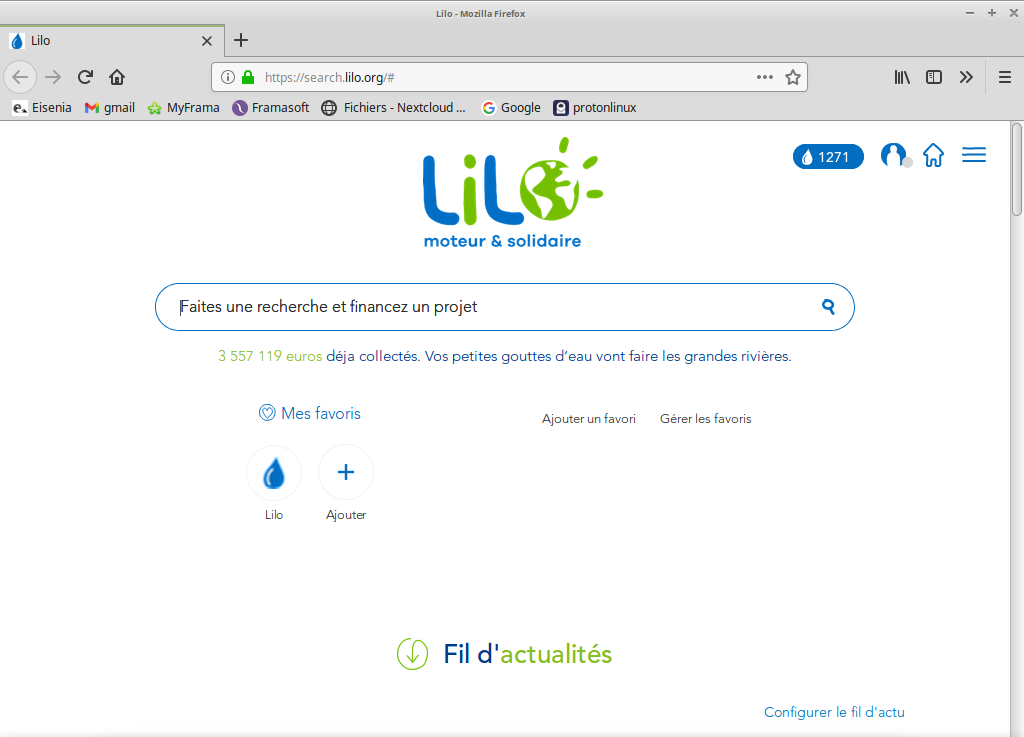
\includegraphics[width=.8\textwidth]{include/lilo.png}
			\caption{Le moteur de recherche Lilo}
			\label{fig:lilo}
		\end{figure}
		\begin{enumerate}
			\item La barre de rechercher.
					Tapez les mots-clés pour votre recherche puis appuyer sur la touche \texttt{Entrée};
			\item Le compteur de gouttes d'eau.
					Visualisez combien de gouttes d'eau vous avez collecté depuis que vous utilisés Lilo;
			\item Le compte Lilo.
					Inscrivez-vous / connectez-vous à votre compte Lilo.
					Ce compte est facultatif;
					Pas besoin d'avoir un compte Lilo pour faire des recherches.
			\item L'accueil.
					Revenez sur la page d'accueil de recherche de Lilo;
			\item Le menu :\newline
			\begin{figure}[h]
				\centering
				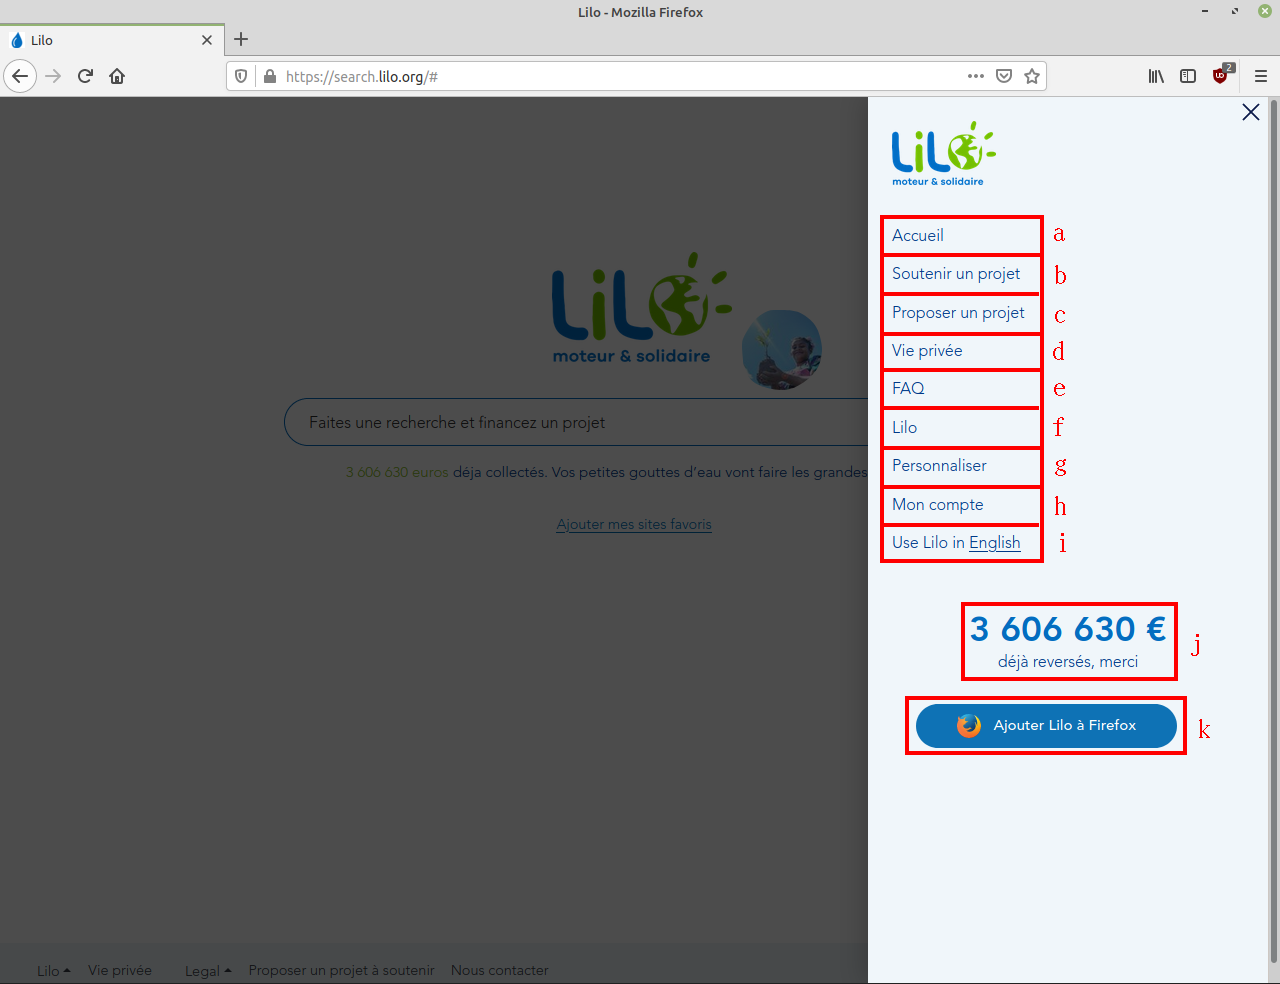
\includegraphics[width=\textwidth]{include/lilo_menu.png}
				\caption{Lilo - Le menu}
				\label{fig:lilomenu}
			\end{figure}
			\begin{enumerate}
				\item \texttt{Accueil} vous permet de revenir à la page de recherche de Lilo.
				\item \texttt{Soutenir un projet} vous permet de sélectionner le (ou les) projet(s) de votre choix en donner vos gouttes d'eau.
				\item \texttt{Proposer un projet} permet à des structures de soumettre leur pojet solidaire à Lilo afin que les internautes puissent leur donner des gouttes d'eau.
				\item \texttt{Vie privée} renvoie vers un descriptif de la gestion des données personnelle par Lilo.
				\item \texttt{FAQ} renvoie vers une page de Questions/Réponses fréquentes.
				\item \texttt{Lilo} renvoie vers une page décrivant le fonctionnement de Lilo.
				\item \texttt{Personnaliser} vous permet d'effectuer des réglages par rapport au moteur de recherche.
				\item \texttt{Mon compte} vous permet de vous connecter ou de vous créer un compte Lilo.
				\item \texttt{Use Lilo in English} vous permet de mettre Lilo en anglais.
				\item Ce compteur affiche le nombre d'euros collectés et reverser par tous les utilisateurs à des projets solidaires.
			\end{enumerate}
		\end{enumerate}
		Si vous le désirez vous pouvez afficher des options dans votre page d'accueil Lilo.
		Elles apparaîtront sous la barre de recherche (\texttt{1}).
		Vous pouvez ajouter à votre page d'accueil :
		\begin{itemize}
			\item Vos favoris.
					Accédez plus rapidement à des pages web en les ajoutant à vos favoris LIlo;
			\item Le fil d'actualité.
					En descendant dans votre page d'accueil, vous pouvez consulter les actualités.
		\end{itemize}	
	\subsection{Effectuer sa première recherche sur Internet}
		Pour effectuer une recherche, rien de plus simple ! 
		Rendez-vous sur votre moteur de recherche, nous prendrons comme exemple Lilo.
		Une fois sur la page d'accueil de Lilo, tapez les mots-clés pour votre recherche.
		Par exemple "Pastèque".
		\begin{figure}[h]
			\centering
			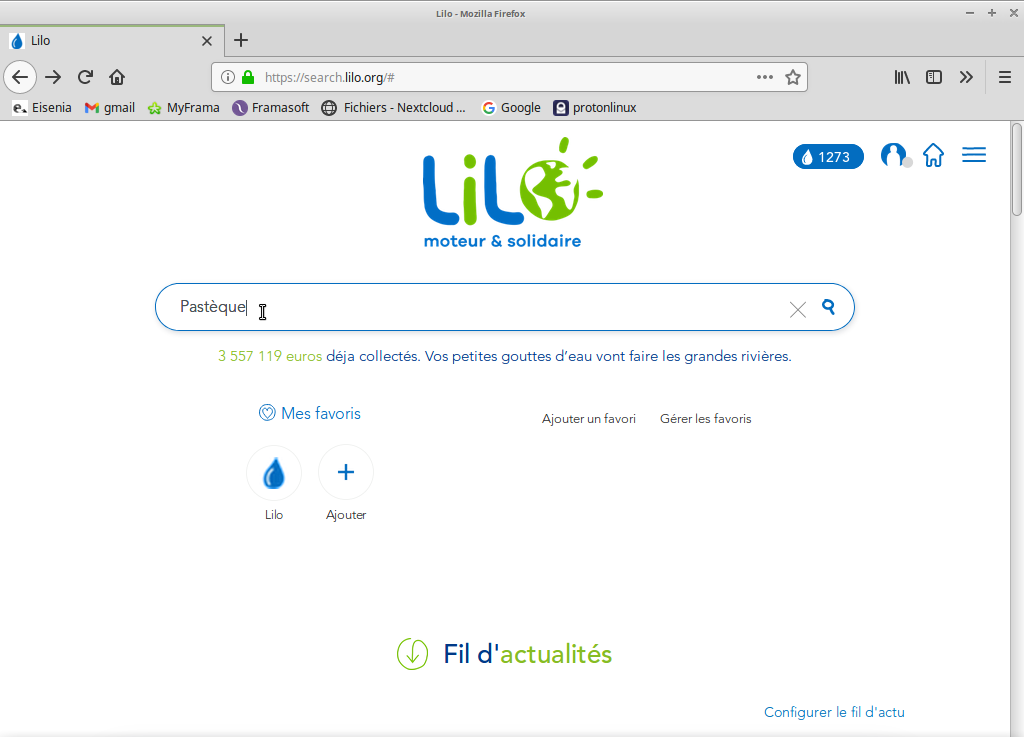
\includegraphics[scale=0.3]{include/pasteque1.png}
			\label{fig:pasteque1}
			\caption{Recherche du mot "Pastèque" dans Lilo}
		\end{figure}
		Appuyer en suite sur la touche \texttt{Entrée} de votre clavier.\par
		Et voilà, le moteur de recherche vous affiche une liste de page web en lien avec le mot clé "Pastèque".
		\begin{figure}[h]
			\centering
			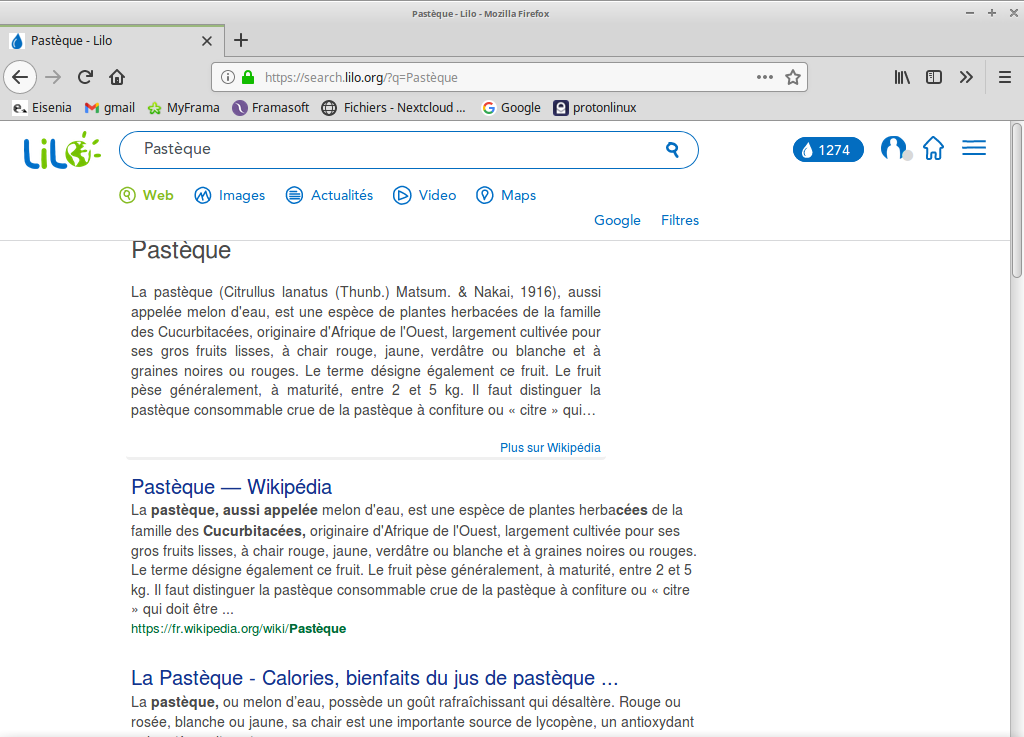
\includegraphics[scale=0.3]{include/pasteque2.png}
			\label{fig:pasteque2}
			\caption{Liste des résultats pour le mot "Pastèque" dans Lilo}
		\end{figure}

\chapter{Mises à jour}\label{sec:maj}
	Dans ce chapitre, nouvs allons aborder le problème des mises à jour;
	Dans un premier temps, nous allons voir l'importance d'effectuer des mises à jour.
	Et dans un second temps. nous allons voir comment effectuer ces mises à jour;
	\section{Pourquoi faire les mises à jour ?}
		Les mises à jour permetten à une application, un logiciel, un système, de corriger certaines erreurs, d'ajouter de nouvelles fonctionnalités ou bien de réparer certaines failles de sécurité.
		Elles sont faites par les développeurs pour être appliquées simplement sur le terminal de tous les utilisateurs.
		Les mises à jour se présentent sous la forme de version à télécharger.\par
		Donc, une mise à jour permet d'améliorer l'ensemble du logiciel.
		D'une part elle peut l'améliorer sur le plan de l'utilisation (nouvelles fonctionnalités, simplification de l'utilisation, correction de bogues, etc.).
		Et d'autre part, elle peut l'améliorer sur le plan de la sécurité et résolvant certaines failles. 
		Par conséquent, il est nécessaire de vérifier régulièrement si des mises à jour sont disponible.
	\section{Effectuer les mises à jour}
		Maintenant, nous allons voir comment faire une mise à jour sur un ordinateur Linux Mint. 
		Notez qu'il vous faut que vous soyez connecter à Internet pour rechercher et installer les mises à jour.\par
		Pour cela :
		\begin{enumerate}
			\item Sur la barre des tâches, à droite, il y a une petite icône en forme de bouclier, cliquez dessus;
			\item Une fenêtre s'ouvre et peut vous afficher différentes informations :
			\begin{itemize}
				\item Si aucune mise à jour n'est à faire, il vous est indiqué que "le système est à jour"
				\item Si des mises à jour sont requisent, alors la liste de ces mises à jour est affichée.
			\end{itemize}
			\item Si rien est coché, cliquez sur "Tout sélectionner";
			\item Cliquez sur le bouton "Installer les mises à jour", votre mot de passe pourra vous être demandé, entrez-le et valider;
			\item Les mises à jour peuvent prendre du temps, ne fermez pas la fenêtre de chargement pendant ce temps.
		\end{enumerate}
		Félicitation ! Votre système et vos logiciels sont à jour !

\chapter{Bonnes pratiques}
	Un ordinateur est un objet très fragile. 
	Il est crucial d'en prendre soin et d'être délicat avec lui.
	Mais pas seulement. 
	Un ordinateur est aussi un outil très puissant, Internet également;
	On peut y trouver toutes sortes d'information mais aussi laisser beaucoup d'informations à notre sujet sans le vouloir.\par
	Dans ce chapitre, nous allons voir les bons gestes à avoir avec son matériel informatique.
	nous allons aussi voir les bons réflexes à adopter en utilisant Internet.
	\section{Entretien du matériel}
		Entretenir votre matériel régulièrement est très important. 
		Cela permettra d'éviter beaucoup de problèmes grâce à de simples gestes.
		\subsection{La poussière}
			Votre ordinateur devient très vite un nid à poussière.
			En effet, lorsqu'il s'agit d'une tour fixe, nous avons tendance à la laisse dans un coin, sous un bureau et on ne la bouge plus.
			Un ordinateur portable n'est pas à l'abri de la poussière non plus.
			Tous les ordinateurs sont exposés au miettes de nourritures, aux poils d'animaux, aux cheveux, etc. Et tout cela s'accumule dans l'ordinateur pouvant entrainer d'une part un bruit très désagréable et d'autres dysfonctionnement/ralentissement de votre système.
			Il faut donc le dépoussiérer régulièrement !\par
			Pour cela, munissez-vous de votre aspirateur ou de votre sèche-cheveux sur un mode souffle froid.
			Si vous avez un compresseur d'air, c'est encore mieux.
			Mettez vous de préférence en extérieur car beaucoup de poussière va sortir de votre ordinateur.
			Si vous ne pouvez pas vous mettre en extérieur, ouvez les fenêtres.
			Débrancher votre ordinateur et ouvrez-le.
			En prenant garde à ne pas abîmer les composants de votre ordinateur, soufflez (ou aspirez) la poussière présente.
			Vous pouvez vous aider d'un chiffon pour attraper la poussière dans les recoins.
		\subsection{La chaleur}
			La chaleur est l'ennemie de votre ordinateur.
			En effet, lorsque le système chauffe trop cela peut entrainer des bogues, des erreurs dûes à des modifications électroniques sous l'effet de la chaleur.
			Mis aussi, à trop haute température, les composants peuvent commencer à fondre.
			C'est d'ailleurs pour éviter ces soucis qu'un ou plusieurs systèmes de refroidissement sont installés dans les ordinateurs. 
			Une bonne pratique est de ne pas laisser votre ordinateur proche d'une source de chaleur (chaffage, cheminée, soleil,...). 
	\section{Sécurité sur internet}
		Internet est une porte ouverte sur beaucoup de connaissances partagées entre tous les utilisateurs.
		Cette outil donne accès à beaucoup d'informations et ce, en très peu de temps.\par
		Mais si internet est si puissant, il reste néanmoins dangereux pour votre ordinateur ainsi que pour vos données personnelles.
		Des personnes malvaillantes peuvent glisser des virus dans des programmes que vous téléchargez.
		Ces virus peuvent être de toutes sortes. Ils peuvent :
		\begin{itemize}
			\item lire ce que vous faites sur votre ordinateurs; 
			\item ouvrir des "portes dérobées" pour extraires des données de votre ordinateur;
			\item altérer des composants logiques ou physiques de votre ordinateur;
			\item bloquer votre ordinateur et vous demander une somme d'argent pour récupérer vos données;
		\end{itemize}
		Il faut donc se protéger de ces virus informatiques.
		Pour cela, il faut tout d'abord utiliser un antivirus, celui-ci effectueras périodiquement des "scans" de votre ordinateur pour vérifier qu'aucun logiciel malvaillant s'y est glissé.
		Evitons de télécharger des fichiers de sources inconnues.
		Sur Linux Mint, pour télécharger un nouveau logiciel il faut passer par la Logithèque, ce qui assure une plus grande sécurité face aux virus.
		Cepandant, vous serez amener à ouvrir et à télécharger des documents provenants d'autres utilisateurs.
		Assurez-vous de toujours connaître votre interlocuteur (par mail par exemple). 
		Si vous ne connaissez pas la personne qui vous envoie un document. ne l'ouvrez pas.\par

\chapter{Avancé}
\section{Utiliser l'invit de commande}\label{sec:utiliserterminal}
	\subsection{Présentation de l'invit de commande}
	\subsection{Les commandes de bases}


\end{document}